\begin{frame}{Vibelavninger}

\small

\begin{columns}[T]

\begin{column}{0.58\textwidth}

\textbf{Regler for vibelavninger:}

\begin{itemize}[]
\item Min. 16 m²
\item Min. 1 pr. ha
\item Min. 40 m til markkant
\item Må ikke gødskes eller sprøjtes
\end{itemize}

\vspace{0.4em}

\textbf{Gavner arter:}

\footnotesize
Vibe, sanglærke, agerhøne, dobbeltbekkasin, engpiber, gul vipstjert, 
rødrygget tornskade, gulspurv, markpiber, vilde bier, humlebier, 
dagsommerfugle, rovbiller, græshopper, pindsvin, musvåge, tårnfalk

\end{column}

\begin{column}{0.40\textwidth}
\centering
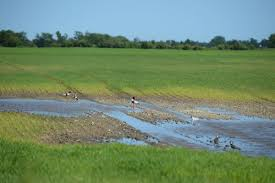
\includegraphics[width=\textwidth]{Billeder/Vildtforvaltning/biotopplantiltag/vibelavninger.jpeg}
\end{column}

\end{columns}

\end{frame}